\section{Решение}

\subsection{Модель 1}

Трёхслойная осесимметричная модель:

{\setlength\tabcolsep{2pt}
\begin{tabular}{rcl}
    первый слой &---& скважина (${0 < r < 1}$) с УЭС ${\rho_\text с = 1}$, \\
    второй слой &---& зона проникновения (${1 < r < r_\text{зп} = 4}$) с УЭС ${\rho_\text{зп} = 4}$, \\
    третий слой &---& пласт (${r > r_\text{зп}}$) с УЭС $\rho_\text{п}$.
\end{tabular}}

\begin{figure}[H]
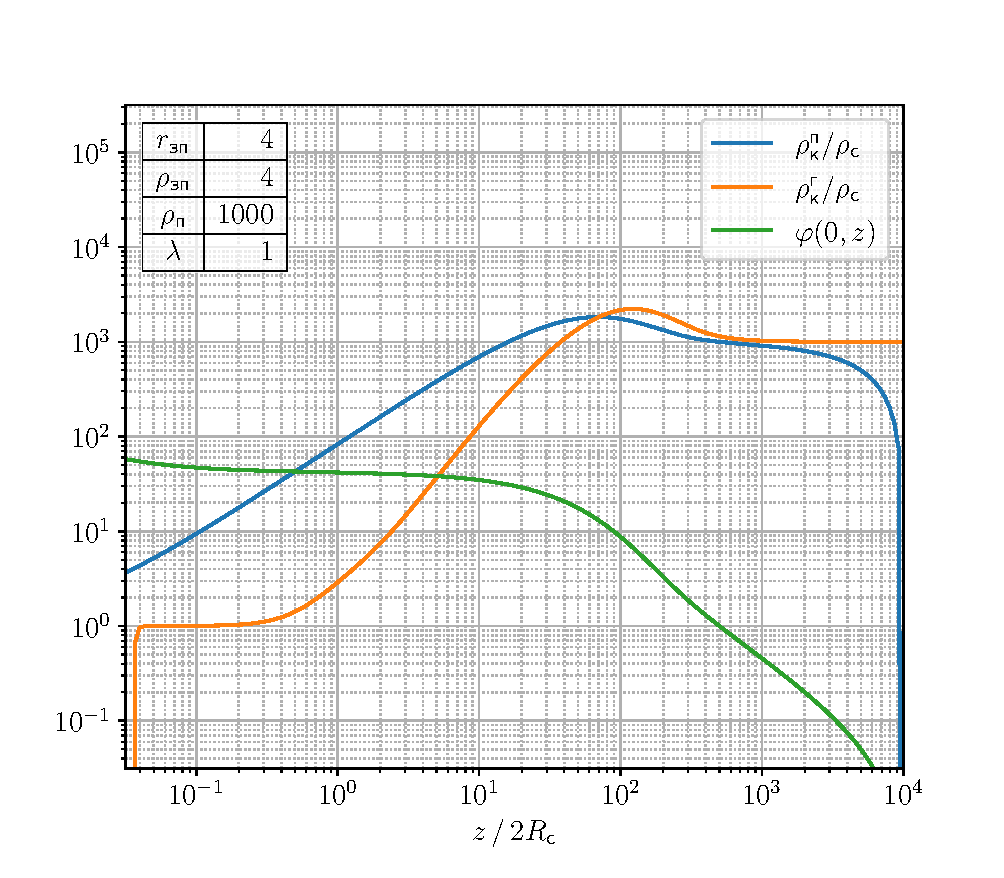
\includegraphics{plot_1_curves}
\caption{График потенциала, кажущихся сопротивлений потециал- и градиент-зондов в скважине}
\label{fig:plot_1_curves}
\end{figure}

Время вычисления решения (рис. \ref{fig:plot_1_curves}) ${1.24 \text{ c } \pm 38.3 \text{ мс}}$, 7 проходов
(${\text{среднее значение} \pm \text{среднеквадратичное отклонение}}$ от 7 проходов, в каждом проходе 1 цикл).

6409 узлов расчетной сетки.

Далее изображены поле, расчетная сетка и решение для палетки с этой расчетной сеткой.

\begin{figure}[H]
\centering
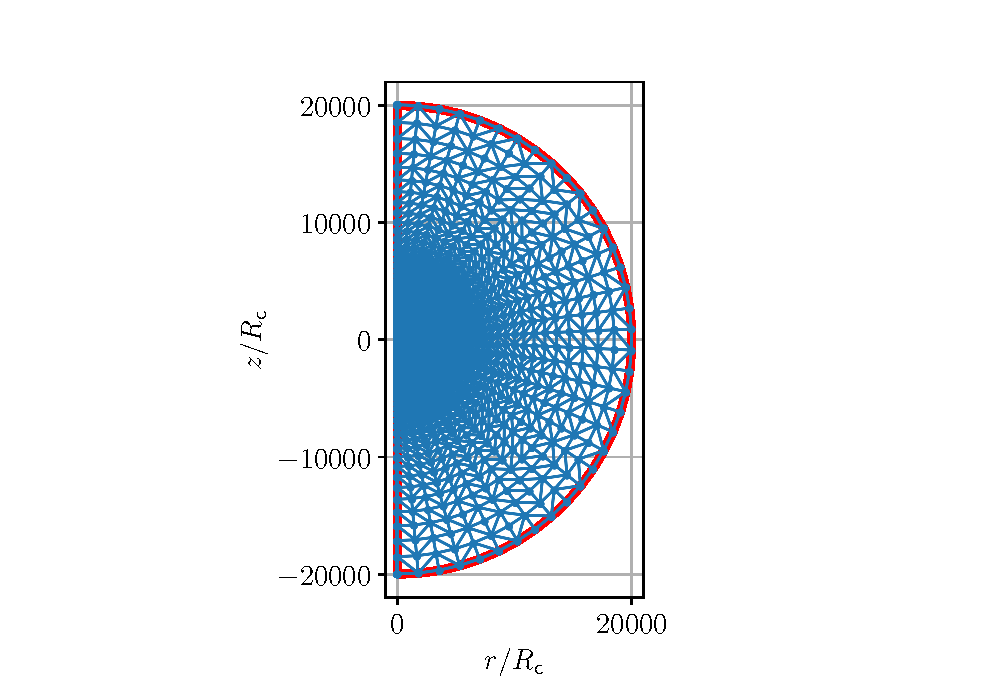
\includegraphics{plot_1_tg_1}
\caption{Триангуляция}
%\label{fig:plot}
\end{figure}

\begin{figure}[H]
\centering
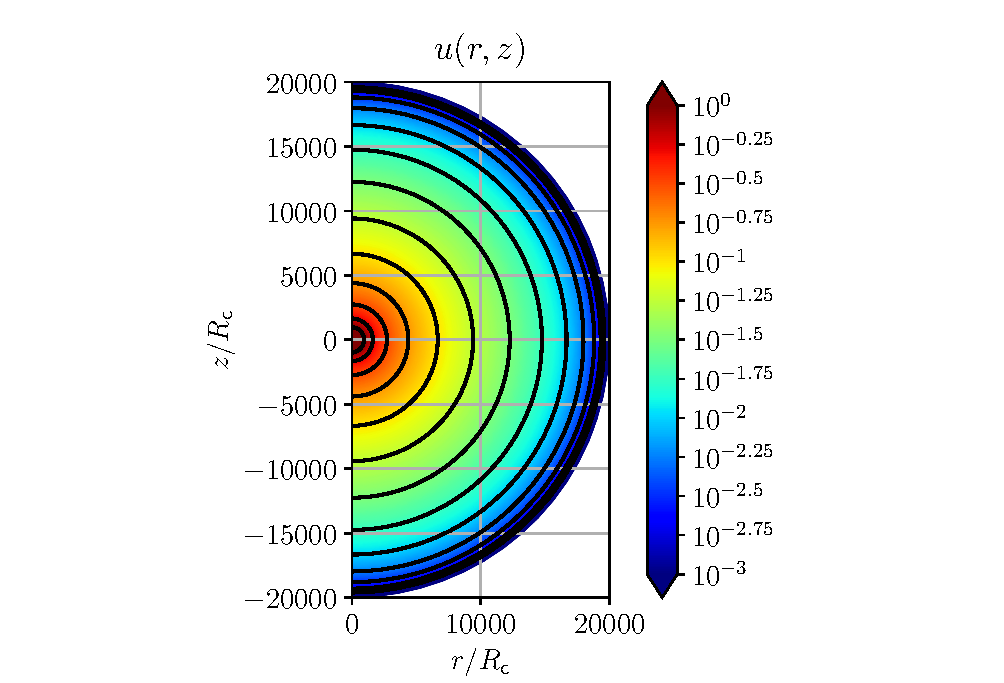
\includegraphics{plot_1_field_1}
\caption{Потенциальное поле}
%\label{fig:plot}
\end{figure}

\begin{figure}[H]
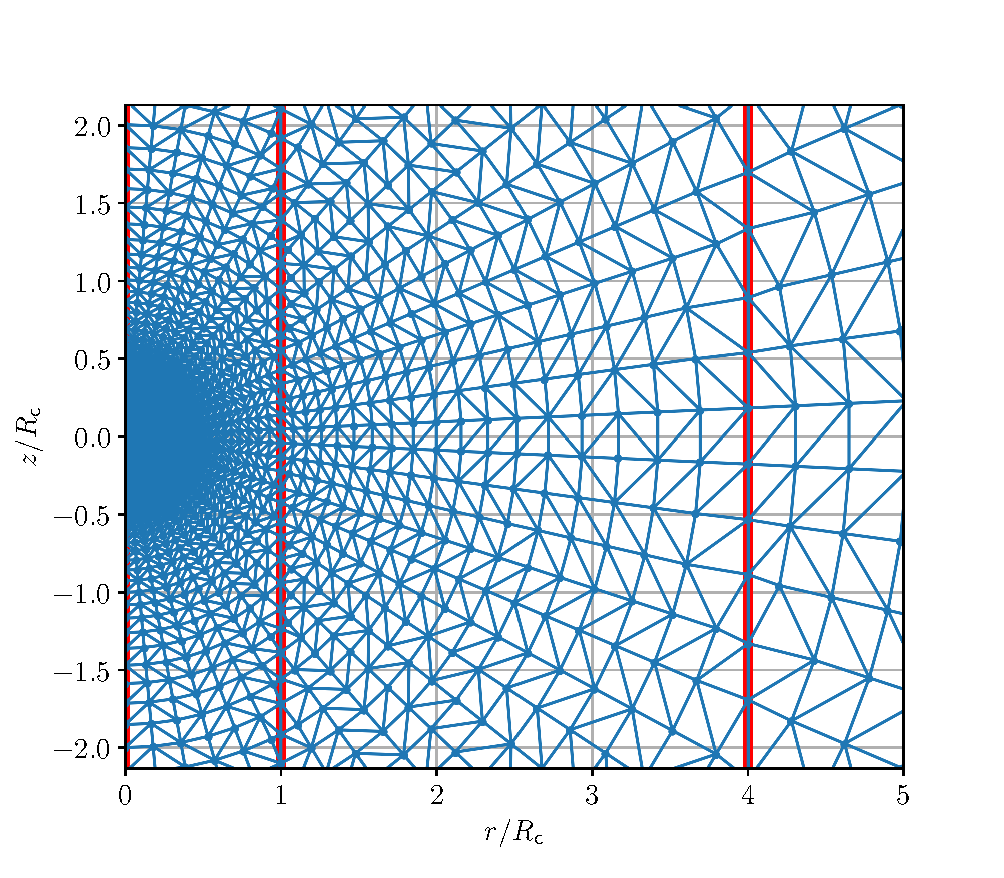
\includegraphics{plot_1_tg_2}
\caption{Триангуляция}
%\label{fig:plot}
\end{figure}

\begin{figure}[H]
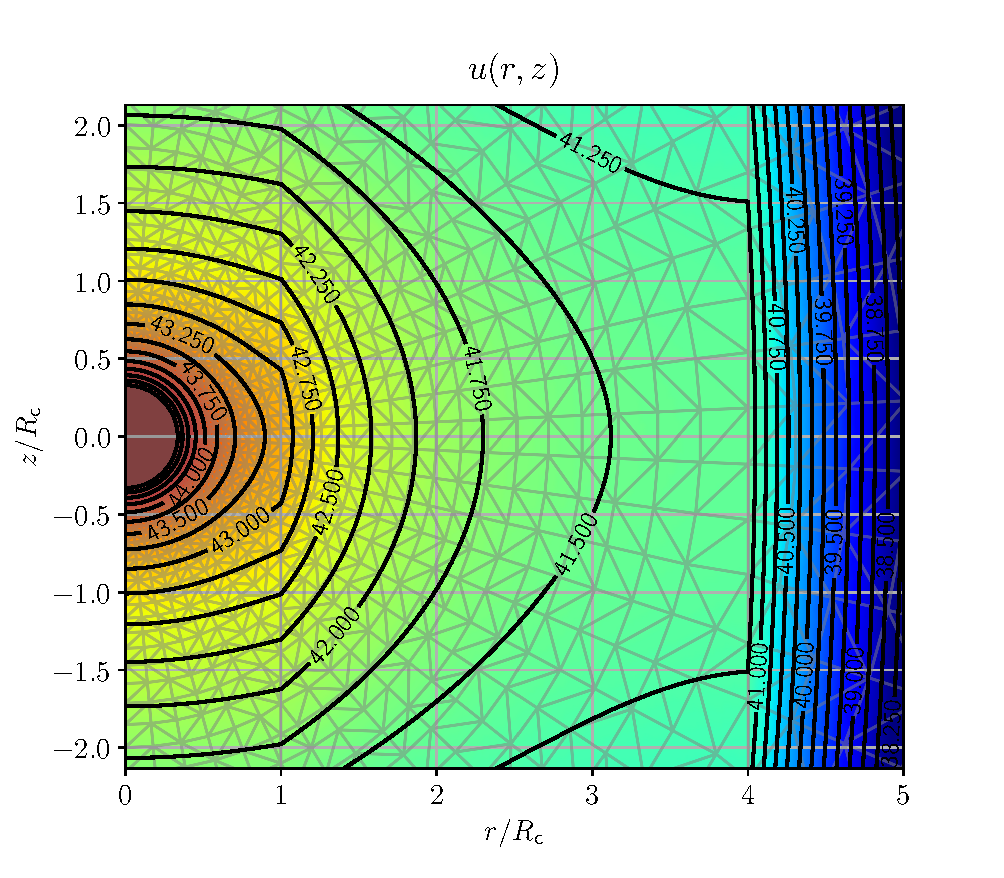
\includegraphics{plot_1_field_2}
\caption{Потенциальное поле}
%\label{fig:plot}
\end{figure}

\begin{figure}[H]
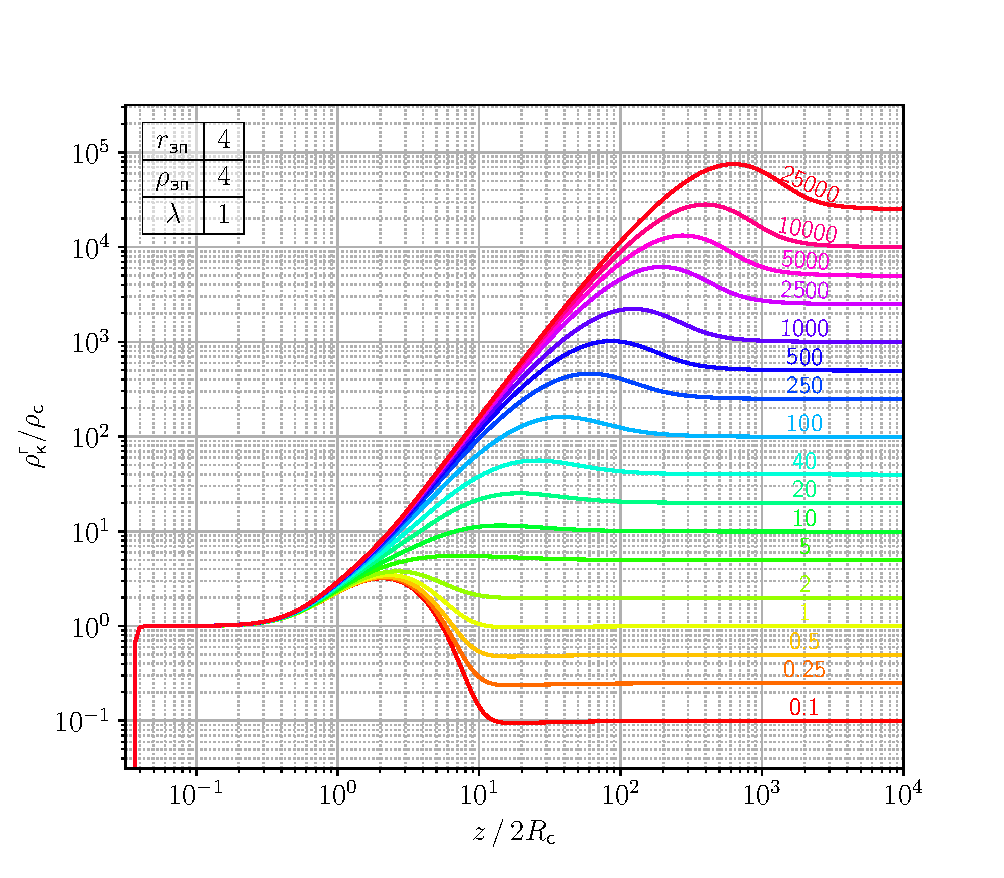
\includegraphics{plot_1_palette}
\caption{Палетка кривых}
\end{figure}

Время вычисления палетки ${18 \text{ c } \pm 159 \text{ мс}}$, 7 проходов.


\begin{figure}[H]
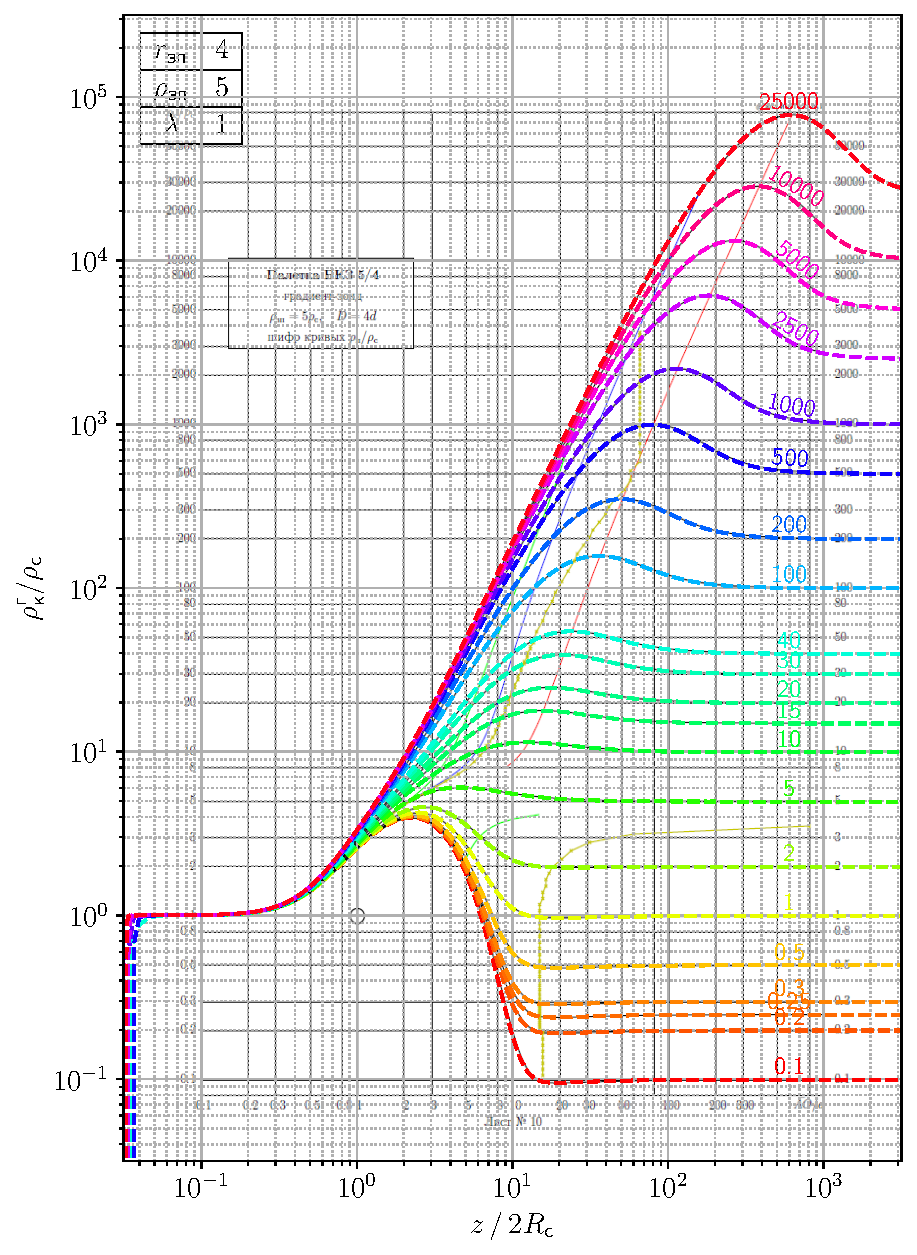
\includegraphics{plot_1_compare}
\caption{Сравнение палетки кривых}
\end{figure}


\newpage
\subsection{Модель 2}

Четырехслойная осесимметричная модель с анизотропией:

\noindent
{\setlength\tabcolsep{2pt} \setlength\intextsep{0mm}
\begin{tabularx}{\linewidth}{r c X}
    первый слой &---& скважина (${0 < r < 1}$)
        с УЭС ${\rho_\text с = 1}$
        с коэффициентом анизотропии ${\lambda_\text{с} = 1}$, \\
    второй слой &---& промытая зона (${1 < r < r_\text{пз} = 2.2}$)
        с УЭС ${\rho_\text{пз} = 4}$
        с коэффициентом анизотропии $\lambda_\text{пз} = \lambda = 1.1$, \\
    третий слой &---& зона проникновения (${r_\text{пз} < r < r_\text{зп} = 5.8}$)
        с УЭС линейная функция от $r$ со значениями ${\rho_\text{зп}(r_\text{пз}) = \rho_\text{пз}}$
        и ${\rho_\text{зп}(r_\text{зп}) = \rho_\text{п}}$
        с коэффициентом анизотропии $\lambda_\text{зп} = \lambda = 1.1$, \\
    четвертый слой &---& пласт (${r > r_\text{зп}}$)
        с УЭС $\rho_\text{п}$
        с коэффициентом анизотропии $\lambda_\text{п} = \lambda = 1.1$.
\end{tabularx}}

\begin{figure}[H]
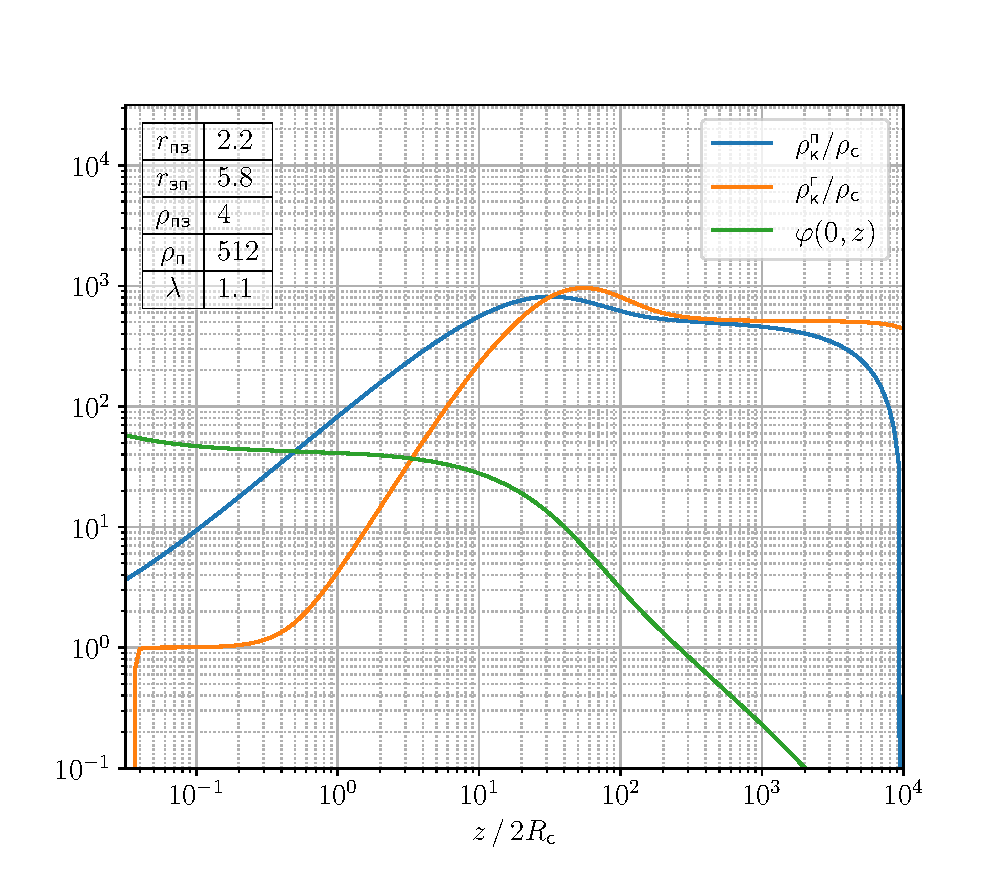
\includegraphics{plot_2_curves}
\caption{График потенциала, кажущихся сопротивлений потециал- и градиент-зондов в скважине}
%\label{fig:plot}
\end{figure}

Время вычисления решения ${1.23 \text{ c } \pm 16.3 \text{ мс}}$, 7 проходов.

6613 узлов расчетной сетки.

Далее изображены поле, расчетная сетка и решение для палетки с этой расчетной сеткой.

\begin{figure}[H]
\centering
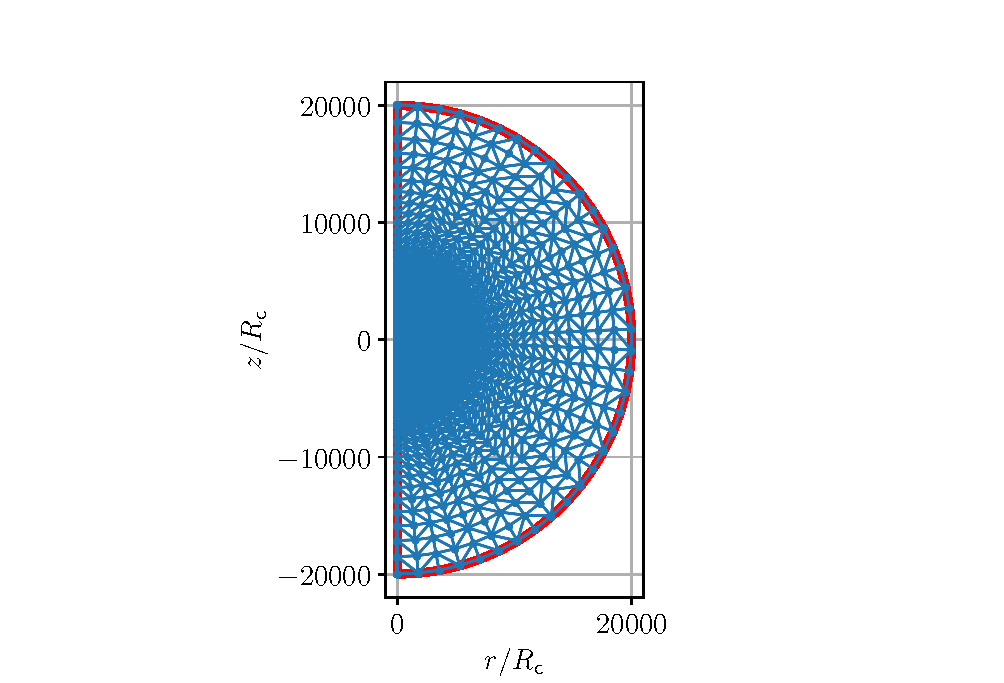
\includegraphics{plot_2_tg_1}
\caption{Триангуляция}
%\label{fig:plot}
\end{figure}

\begin{figure}[H]
\centering
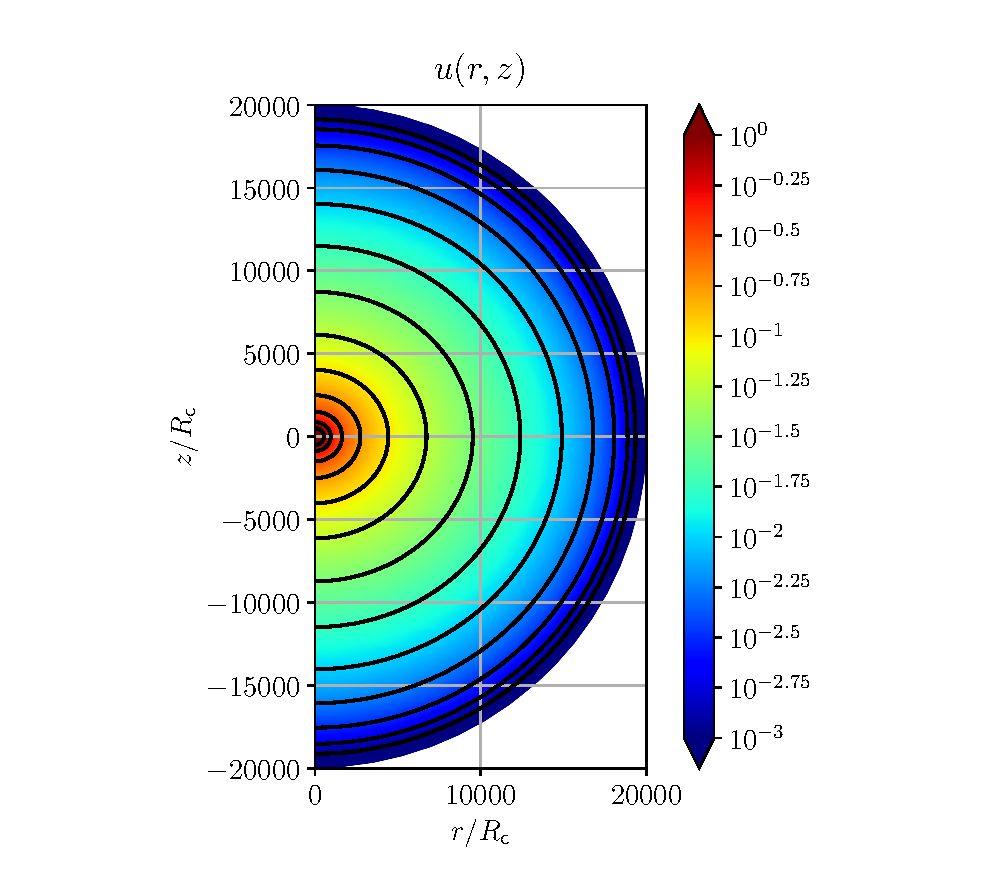
\includegraphics{plot_2_field_1}
\caption{Потенциальное поле}
%\label{fig:plot}
\end{figure}

\begin{figure}[H]
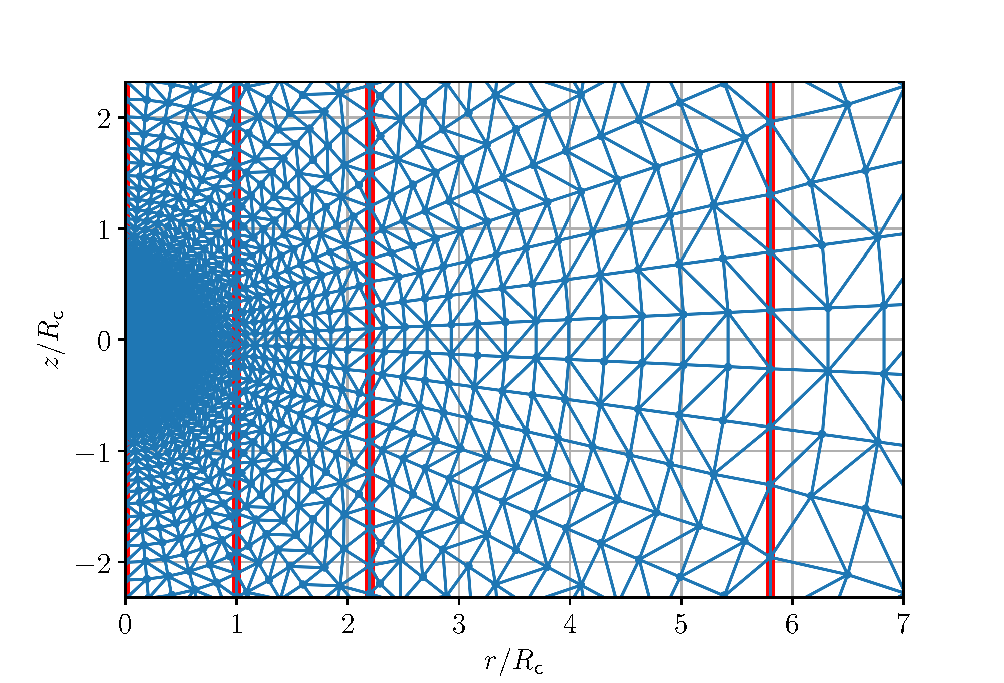
\includegraphics{plot_2_tg_2}
\caption{Триангуляция}
%\label{fig:plot}
\end{figure}

\begin{figure}[H]
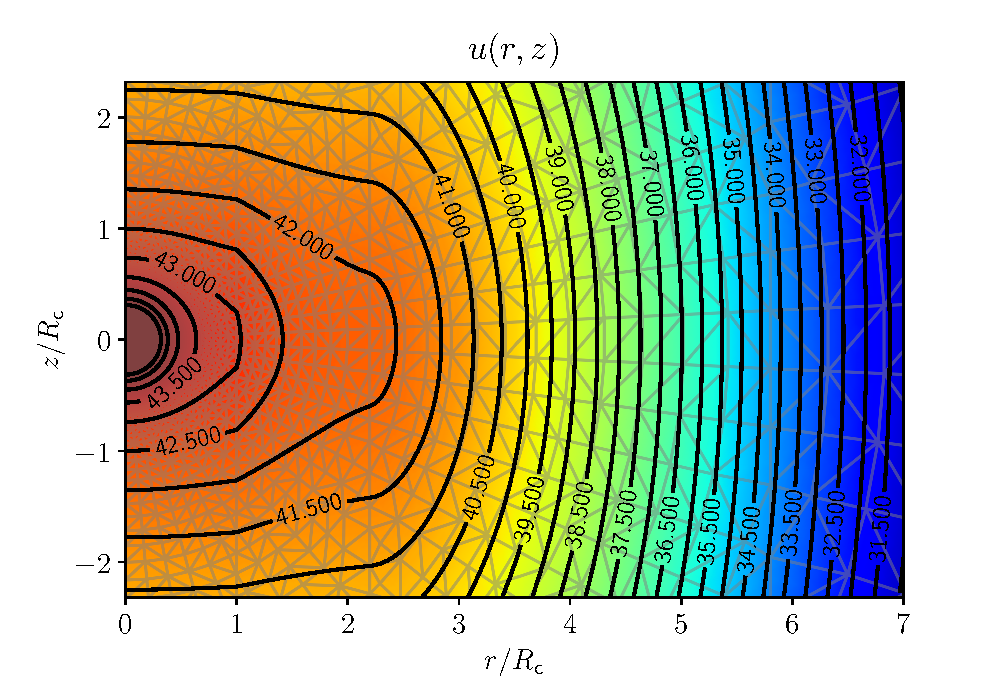
\includegraphics{plot_2_field_2}
\caption{Потенциальное поле}
%\label{fig:plot}
\end{figure}

\begin{figure}[H]
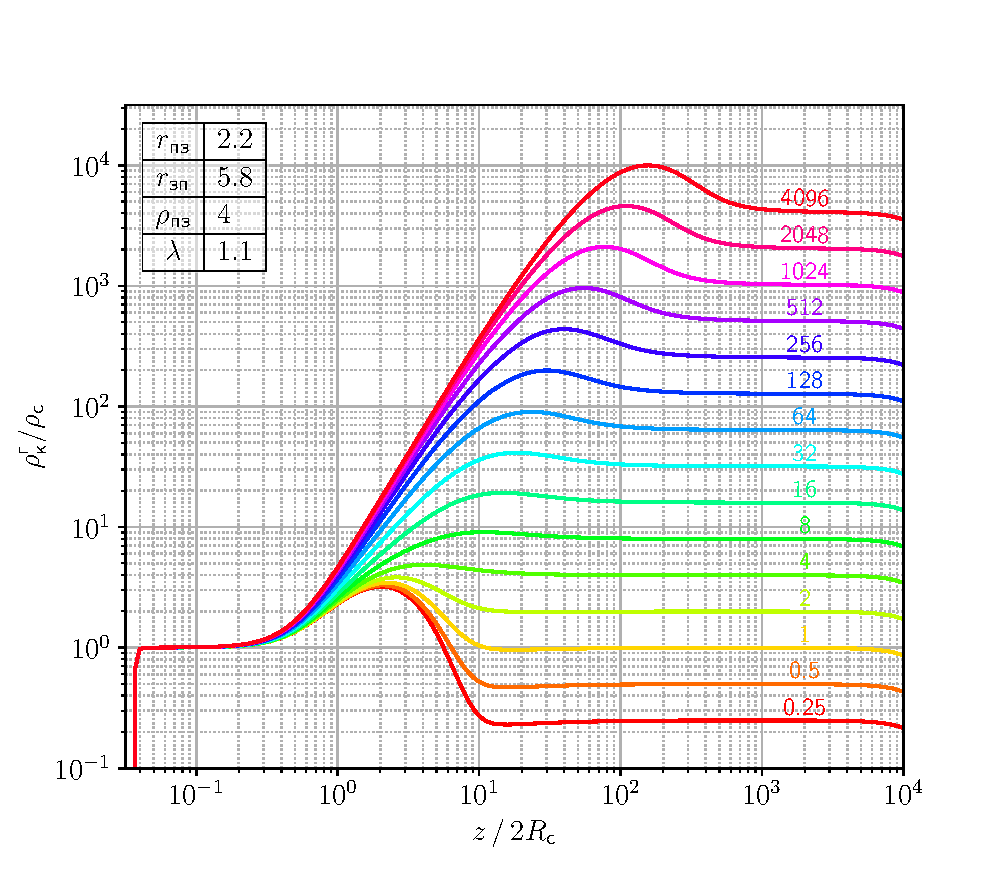
\includegraphics{plot_2_palette}
\caption{Палетка кривых}
\end{figure}

Время вычисления палетки ${16.5 \text{ c } \pm 176 \text{ мс}}$, 7 проходов.

\begin{figure}[H]
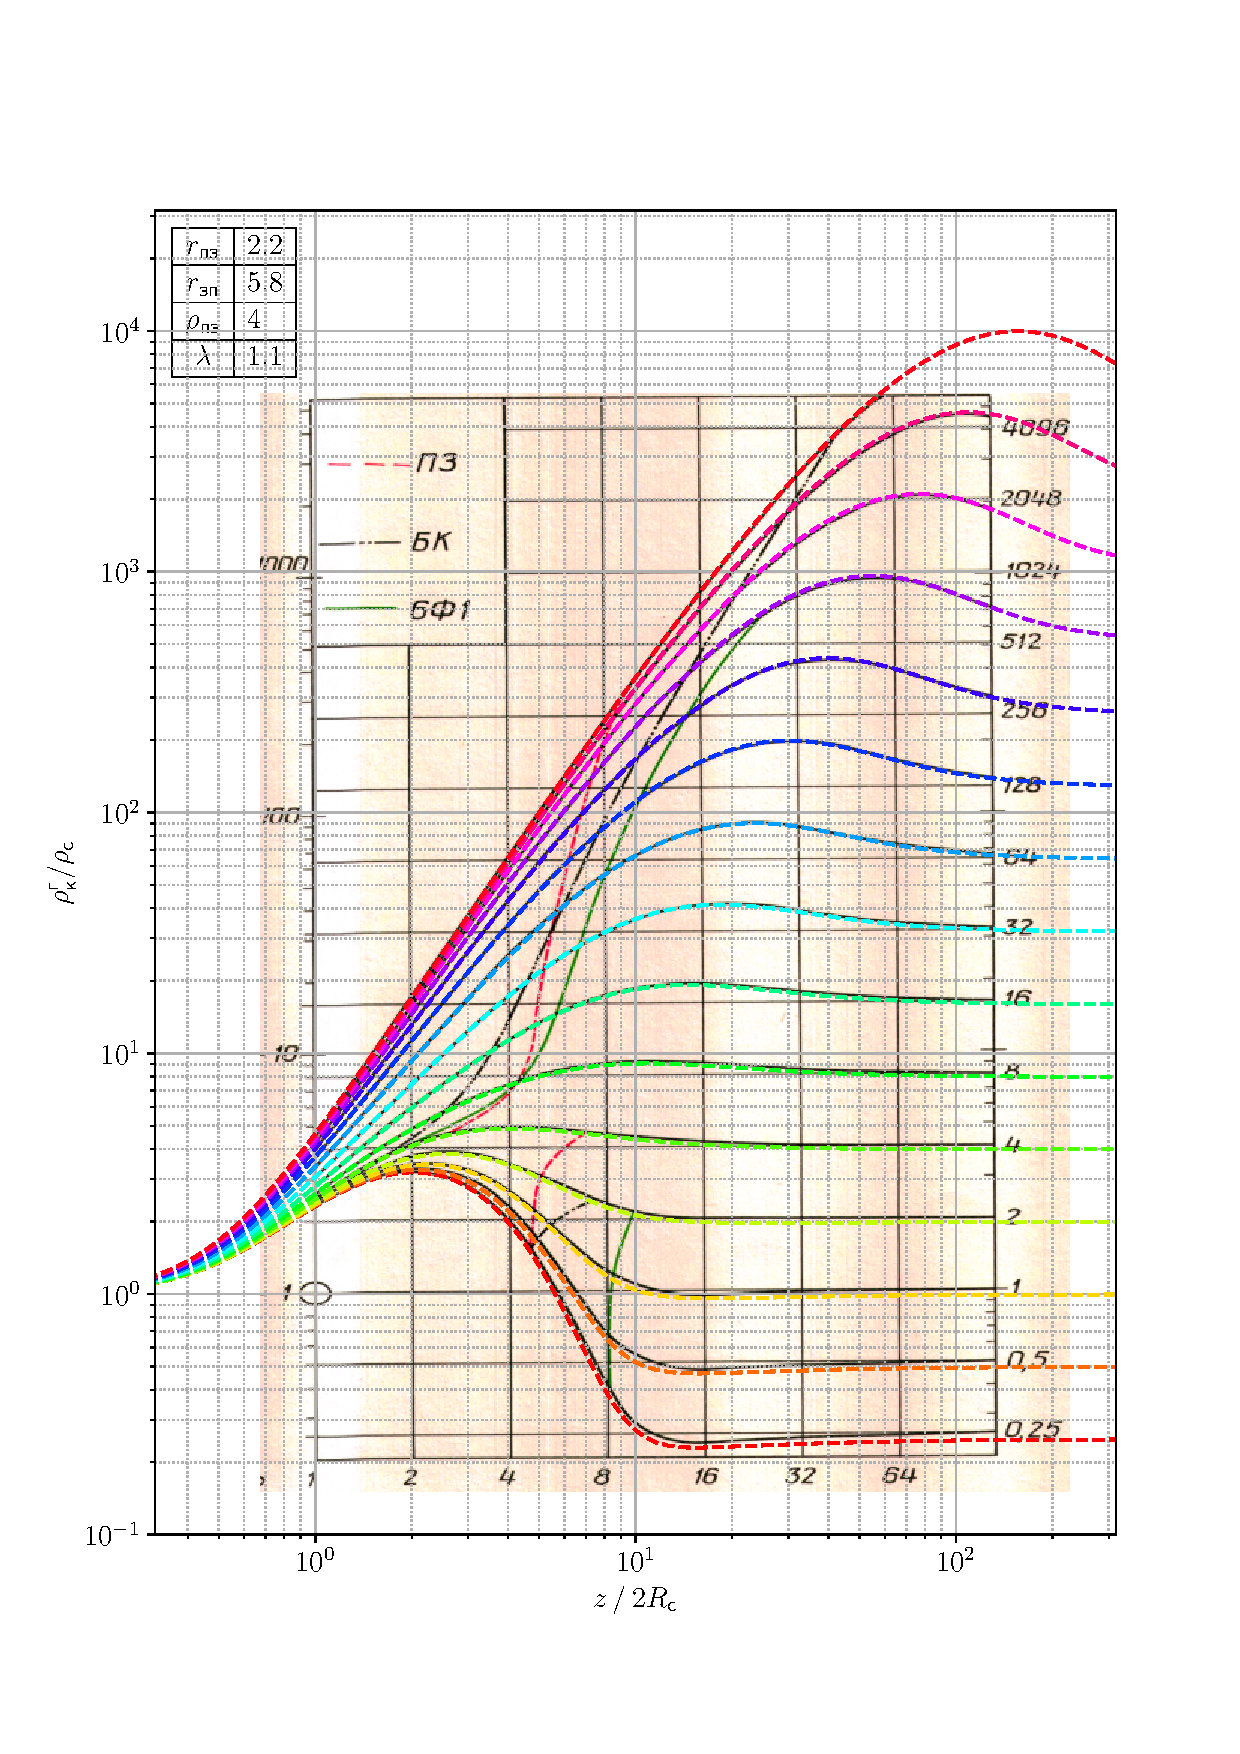
\includegraphics{plot_2_compare}
\caption{Сравнение палетки кривых}
\end{figure}

\clearpage
